%
% File naaclhlt2018.tex
%
%% Based on the style files for NAACL-HLT 2018, which were
%% Based on the style files for ACL-2015, with some improvements
%%  taken from the NAACL-2016 style
%% Based on the style files for ACL-2014, which were, in turn,
%% based on ACL-2013, ACL-2012, ACL-2011, ACL-2010, ACL-IJCNLP-2009,
%% EACL-2009, IJCNLP-2008...
%% Based on the style files for EACL 2006 by 
%%e.agirre@ehu.es or Sergi.Balari@uab.es
%% and that of ACL 08 by Joakim Nivre and Noah Smith

\documentclass[11pt,a4paper]{article}
\usepackage[hyperref]{naaclhlt2018}
\usepackage{times}
\usepackage{latexsym}
\usepackage{soul}
\usepackage{tikz}
\usepackage{amsmath}
\usepackage{booktabs}

\usepackage{url}


\usepackage{graphicx}
\graphicspath{{figures/}}
\DeclareGraphicsExtensions{.png,.eps,.pdf,.jpg}

\DeclareMathOperator{\wsim}{sim}

%\aclfinalcopy % Uncomment this line for the final submission
%\def\aclpaperid{***} %  Enter the acl Paper ID here

%\setlength\titlebox{5cm}
% You can expand the titlebox if you need extra space
% to show all the authors. Please do not make the titlebox
% smaller than 5cm (the original size); we will check this
% in the camera-ready version and ask you to change it back.

\newcommand\BibTeX{B{\sc ib}\TeX}

\title{Using Paraphrases to Cluster and Order Adjectives by Intensity:\textbf{}\\Phenomenal == absolutely amazing, so phenomenal $>$ amazing}

% Authors: Veronica, Xiao, Ellie, CCB, Anne, and Marianna
\author{First Author \\
  Affiliation / Address line 1 \\
  Affiliation / Address line 2 \\
  Affiliation / Address line 3 \\
  {\tt email@domain} \\\And
  Second Author \\
  Affiliation / Address line 1 \\
  Affiliation / Address line 2 \\
  Affiliation / Address line 3 \\
  {\tt email@domain} \\}

\date{}

\begin{document}
\maketitle
\begin{abstract}
Adjectives like {\it fine}, {\it good}, {\it great}, and {\it phenomenal} all describe quality, but differ in intensity (i.e., {\it fine} $<$ {\it good} $<$ {\it great} $<$ {\it phenomenal}). Understanding these intensity differences is a necessary part of reasoning about natural language. We present a method to automatically learn the relative relationship of scalar adjectives. Our approach is based on pairwise adjective intensity relationships that are inferred by analyzing pairs of adjectival paraphrases from the Paraphrase Database (\href{http://paraphrase.org}{http://paraphrase.org}). We propose a method to construct clusters of adjectives pertaining to a single attribute (e.g. food quality), and to rank adjectives within clusters according to their relative intensities. We apply the method to predicting the sentiment polarity of Twitter posts.
\end{abstract}

\section{Introduction}

Semantically similar adjectives are rarely fully interchangeable in context. For example, although \textit{good} and \textit{great} are synonyms, \textit{the cookies were good} does not imply that \textit{the cookies were great}. In fact, in the case of \textit{fine} and \textit{outstanding}, \textit{the cookies were outstanding} implies quite a different sentiment than \textit{the cookies were fine}. \textit{Fine}, \textit{good}, \textit{great}, and \textit{outstanding} are not interchangeable because they differ in intensity; a native English speaker understands that \textit{fine} $<$ \textit{good} $<$ \textit{great} $<$ \textit{outstanding}.

Knowing the scalar ordering of adjectives has several applications. For example, adult language learners may struggle to learn subtle semantic differences between similar adjectives, and software for language learning could include graphical representations of scalar adjective scales to facilitate lexical acquisition \cite{sheinman2013large}. Scalar adjective intensity rankings are also potentially useful for several NLP tasks, including question answering \cite{demarneffe:10}, and textual inference, including recognizing textual entailment \cite{Dagan2006}. In this work, we demonstrate their potential to improve scores on the task of sentiment analysis \cite{Pang:2008:OMS:1454711.1454712}. 

% A more concrete task that scalar adjective scales would aid is identifying spam product reviews. A spam review is an online review whose purpose is to deceive or confuse potential buyers. Spam product reviews typically include more intense (either very positive or very negative) adjectives. Thus, adjectives' positions (high or low) on semantic intensity scales might be useful in a classifier for detecting spam \cite{}.

The relative intensities of adjectives are not included in current lexical resources. Both thesauri and WordNet \cite{Miller:1995:WLD:219717.219748} include specific types of semantic relations, including synonymy, antynomy, and hyponymy. Vector-based representations of word semantics (e.g., \texttt{word2vec} \cite{word2vec}) capture a broader notion of semantic similarity between adjectives. None of these resources, however, provide the relative intensity of pairs or sets of adjectives. 

Our work is divided into two tasks: (1) Retrieve clusters of adjectives that belong on a single intensity scale, given a seed (\textit{adjective,noun}) pair to guide the search, and (2) order adjectives within each cluster by relative intensity. We approach both tasks by inferring relationships between adjectives by analyzing paraphrases from the Paraphrase Database (PPDB) \cite{pavlick-EtAl:2015:ACL-IJCNLP3}. For example, if \textit{very good} is a paraphrase for \textit{great} in PPDB, this is evidence that \textit{good} and \textit{great} modify the same attribute and therefore belong on the same intensity scale. Further, since \textit{very} intensifies adjectives that it modifies, we infer that \textit{good} is less intense than \textit{great}. We construct a graph that encodes these pairwise relationships, and use it as the basis for clustering adjectives by attribute and ordering them by intensity.

Previous work has focused on clustering semantically similar adjectives \cite{hatzivassiloglou:93,shivade:15}. Our approach is unique in that it uses paraphrases to infer pairwise intensity relationships between adjectives and in that it uses an explicit graph structure to represent all known relationships. Previous work \cite{demarneffe:10,demelo:13,shivade:15} has also focused on ranking sets of semantically similar adjectives by intensity.

We evaluate our adjective clusters and rankings against ground-truth clusters and rankings. We construct the ground-truth clusters using human judgements gathered from Amazon Mechanical Turk (MTurk) HITs, and borrow the ground-truth rankings from a previously-published dataset \cite{demelo:13}. Then, we evaluate our system extrinsically by showing how it can be useful in the task of aspect-based sentiment analysis \cite{pontiki2014semeval,pontiki2016semeval}, where the goal is to identify the sentiment expressed for specific aspects of items mentioned in a product review.

\section{Related work}

\subsection{Clustering semantically similar adjectives}

\newcite{hatzivassiloglou:93} describe an algorithm for clustering adjectives that extracts syntactically related words from a large, parsed corpus and quantifies the similarity and dissimilarity of each pair of evaluated adjectives. Clusters are constructed by initially selecting a random partition and improving the partition iteratively using an objective function that considers the similarity and dissimilarity of clusters' members. 

\newcite{shivade:15} use the \textit{k}-means clustering method to generate adjective clusters. Their distance metric is cosine similarity between \texttt{word2vec} vectors. 

Both \newcite{hatzivassiloglou:93} and \newcite{shivade:15} use ``hard" clustering algorithms -- algorithms that produce disjoint clusters, thus preventing words with multiple meanings from appearing in multiple clusters. By contrast, ``soft" clustering algorithms accommodate polysemous words. \newcite{shivade:15} explicitly leave deriving a soft clustering approach as a separate research problem.

\subsection{Ranking adjectives by intensity}

% PAPER 2

% Additional related work suggested by Chris
%\newcite{sheinman2009adjscales} Rank adjectives using lexical-semantic patterns that indicate pairwise intensity relationships using the Web as a corpus (AdjScales method). Perform exhaustive pairwise comparisons between all adjectives in the cluster to establish a total ordering of adjectives. Propose usefulness of intensity rankings of adjectives for language learners. 
% \newcite{sheinman2012refining} Apply AdjScales method to WordNet dumbbells. Discussion of the origins of WordNet and of the structure of WordNet dumbbells. Provides additional potential applications of knowing the relative intensity rankings of adjectives. (Very little additional content beyond their previous paper.)

\newcite{demarneffe:10} use scalar relationships between adjectives to infer the answers to polar questions that do not explicitly contain a ``yes" or ``no" word (e.g., \textit{Do you think it's a good idea? I think it's an excellent idea.}). Thus, their interest is primarily in scalar relationships between pairs of adjectives. The relative intensity of adjectives is inferred by finding the adjectives in a corpora of online reviews and comparing the reviews' associated numerical ratings. 

\newcite{demelo:13} infer pairwise intensity relationships using linguistic patterns found in a large corpus and then determine a global ordering of adjectives using a Mixed Integer Linear Program (MILP). Frequency information for the MILP is gathered from the Google N-Grams dataset. They use adjective clusters based on WordNet \textit{dumbbells}, which each consist of two antonyms (the poles) and several other adjectives that are semantically similar to one of the poles. \newcite{shivade:15} also apply \newcite{demelo:13}'s MILP implementation, gathering frequency data from the PubMed corpus to rank the adjectives in their clusters. 

% Both methods use large corpora to inform the pairwise and global rankings of adjectives.  

% \iffalse
% \cite{hatzivassiloglou:93} 

% Uses syntactic patterns

% Clusters adjectives that are on single intensity scale but doesn't rank them

% Use a large labeled text corpora

% Uses no semantic information about adjectives

% Uses a multi-step algorithm that quantifies similarity and dissimilarity between every pair of evaluated adjectives first by identifying 

% Targets a small set of adjectives

% Clusters using similarity and dissimilarity measures

% % PAPER 1

% \cite{demarneffe:10} seeks to determine the scalar relationship between adjectives in order to infer the answer to polar questions that do not explicitly contain a ``yes" or ``no" word (e.g., \textit{Do you think it's a good idea? I think it's an excellent idea.}).
% Their method was successful but their corpora was small in size

% They seek to identify only pairwise intensity relationships

% Their method is very different from ours -- they infer the intensity of adjectives by associating finding them in a review with an associated rating. 

% They utilize two corpora: CNN interview transcripts (to find questions) and online reviews from IMDB (to determine intensity of adjectives)

% Was it good? It was provocative - 
% uses lexico-semantic patterns in polar questions (questions to which the answer is yes or no)
% uses a corpora of online reviews and broad web searches
% seeks to use context to determine answers to indirect questions (used to drive pragmatic inference in dialogue)
% uses the scalar relationship between adjectives to infer the answer to polar questions
% They hypothesize that uncertainty results when the main predication in the question and the main predication in the answer have no entailment relationship (have no "reliable scalar relationship")



% % PAPER 0

% Good, Great, Excellent - 
% uses lexico-semantic patterns that suggest an intensifying (``weak-strong pattern") or de-intensifying (``strong-weak pattern") relationship (e.g., "good but not great", "hot and almost scorching") 
% also uses transitivity relationships
% uses a Mixed Integer Linear Program (MILP) 
% uses a web-scale corpus of data

% Depends on a manually created dataset (WordNet or FrameNet)

% Uses WordNet dumbbells to get the original clusters for adjectives

% % PAPER 3

% \cite{shivade:15}

% Uses an optimized KMeans to cluster adjectives (using cosine 

% % Final thoughts

% None use a graph-based approach

% corpus-based vs. manual-resource-based
% \fi

\section{Constructing an adjective graph}

Our basis for extracting same-aspect adjectives and ordering them by intensity is a graph of adjectives and their relationships. In the graph, which we call \textit{JJGraph}, nodes are adjectives, and edges connect adjectives that become paraphrases when an adverb is prepended to one adjective in the pair. Here we discuss \textit{JJGraph}'s construction and attributes.

\subsection{Data: Paraphrase Database}

\textit{JJGraph} is built from paraphrases in the Paraphrase Database (PPDB) \cite{pavlick-EtAl:2015:ACL-IJCNLP3}. Each pair of connected nodes corresponds to an adjectival paraphrase (e.g., \textit{very tall} $\leftrightarrow$ \textit{large}), where one `phrase' is a single-word adjective and the other is an multi-word adjectival phrase containing an adverb and adjective. Figure \ref{fig:adjexamples} gives examples of paraphrase pairs encoded in the graph. In total, we use 36,756 adjective paraphrases that contain 21,701 unique adjectives and 610 unique adverbs.  

\begin{figure}[t]
\begin{center}
\begin{tabular}{| l c l |}
 \hline
 \textit{particularly pleased} & $\leftrightarrow$ & \textit{ecstatic} \\ 
 \hline
 \textit{quite limited} & $\leftrightarrow$ & \textit{restricted} \\ 
 \hline 
 \textit{rather odd} & $\leftrightarrow$ & \textit{crazy} \\
 \hline
 \textit{so silly} & $\leftrightarrow$ & \textit{dumb} \\
 \hline
 \textit{completely mad} & $\leftrightarrow$ & \textit{crazy} \\
 \hline
\end{tabular}
\end{center}
\caption{Sample paraphrases in PPDB}
\label{fig:adjexamples}
\end{figure} 

\subsection{Adverbs}

Our method uses adjective paraphrases from PPDB that contain intensifying adverbs. An \textbf{intensifying adverb} semantically strengthens the adjective that it modifies. For example, \textit{very} and \textit{so} are intensifying adverbs. In contrast, a \textbf{de-intensifying adverb} semantically weakens the adjective that it modifies. For example, \textit{slightly} and \textit{somewhat} are de-intensifying adverbs. 

We use paraphrases to make pairwise intensity relations. For example, since \textit{so wonderful} is a paraphrase for \textit{brilliant}, we infer that \textit{wonderful} $<$ \textit{brilliant}. %Similarly, since \textit{slightly tricky} is a paraphrase for \textit{hard}, we infer that \textit{hard} $<$ \textit{tricky}. 

\begin{figure}[t]
	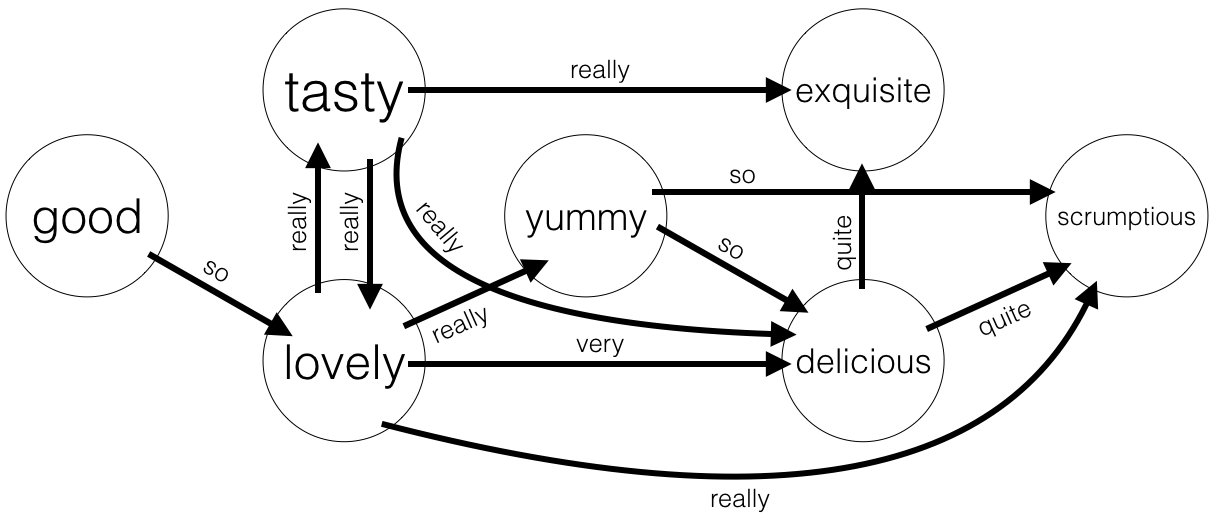
\includegraphics[width=\columnwidth]{graph.png}
	\caption{Directed graph structure}
\end{figure} 


\subsection{Identifying intensifying adverbs}

We used an iterative process to identify intensifying adverbs (Figure 3), and then used paraphrases containing the identified intensifying adverbs to construct \textit{JJGraph}. 

\begin{figure}[t]
	\begin{center}
	\begin{tabular}{ c | c c c c | }
		\cline{2-5}
 		Round 1 & \textbf{very} & hard & $\Leftrightarrow$ & harder \\ 
 		& \textbf{kinda} & hard & $\Leftrightarrow$ & harder \\  
 		& \textbf{so} & hard & $\Leftrightarrow$ & harder \\
		& \textbf{pretty} & hard & $\Leftrightarrow$ & harder \\  
		\cline{2-5}
		
		\multicolumn{1}{c}{} & $\Downarrow$ & & & \multicolumn{1}{r}{} \\ 
		
		\cline{2-5}
 		Round 2 & very & \textit{pleasant} & $\Leftrightarrow$ & \textit{delightful} \\ 
 		& kinda & \textit{hard} & $\Leftrightarrow$ & \textit{tricky} \\  
 		& so & \textit{wonderful} & $\Leftrightarrow$ & \textit{brilliant} \\
		& pretty & \textit{simple} & $\Leftrightarrow$ & \textit{plain} \\
		\cline{2-5}
		
		\multicolumn{1}{r}{} & $\Downarrow$ & & \multicolumn{1}{c}{$\Downarrow$} \\
		
		\cline{2-5}
 		Round 3 & \textbf{more} & pleasant & $\Leftrightarrow$ & delightful \\ 
 		& \textbf{really} & hard & $\Leftrightarrow$ & tricky \\  
 		& \textbf{truly} & wonderful & $\Leftrightarrow$ & brilliant \\
		& \textbf{fairly} & simple & $\Leftrightarrow$ & plain \\
		\cline{2-5}
	\end{tabular}
	\end{center}
	\caption{Iterative process for identifying adverbs}
\end{figure}

First, we identified pairs of phrases in which one phrase contained the base form of an adjective (e.g., \textit{hard}) and the other phrase contained either the comparative or superlative form of the same adjective (e.g., \textit{harder} or \textit{hardest}). Such pairs were identified by lemmatizing the longer word in the pair (\textit{harder}), and comparing the lemma (\textit{hard}) to the shorter word in the pair (\textit{hard}) for equality. NLTK's \texttt{WordNetLemmatizer} was used for lemmatizing (\newcite{nltk}). 

By definition, the base form of an adjective is less semantically intense than both its comparative and superlative forms (e.g., \textit{hard} $<$ \textit{harder} $<$ \textit{hardest}). Thus, the adverb that precedes the base form of the adjective is presumed to be an intensifying adverb. 

Next, we found pairs of phrases that included the adverbs found in Round 1. For example, whereas in Round 1 we identified \textit{very} and \textit{pretty} as intensifying adverbs, we found in Round 2 that \textit{pleasant} and \textit{delightful} and that \textit{simple} and \textit{plain} were also related by \textit{very} and \textit{pretty}, respectively. That is, \textit{pleasant} $<$ \textit{delightful} and \textit{simple} $<$ \textit{plain}. 

Finally, in Round 3, we identified additional intensifying adverbs by finding pairs of phrases with the words identified in Round 2. For example, in Round 2 we found the patterns \textit{[adverb] pleasant} $\leftrightarrow$ \textit{delightful} and \textit{[adverb] simple} $\leftrightarrow$ \textit{plain}, so in Round 3 we found all other pairs of phrases that fit those patterns (e.g., \textit{more pleasant} $\leftrightarrow$ \textit{delightful}, \textit{fairly simple} $\leftrightarrow$ \textit{plain}). The adverbs in these phrases (e.g., \textit{more}, \textit{fairly}) are intensifying.

In total, we identified 677 intensifying adverbs using this process. We then used the set of intensifying adverbs to search for suitable paraphrases to include in \textit{JJGraph}.

\subsection{Choosing a graph representation}

The transitivity of scalar relationships (e.g., if $A < B$ and $B < C$, then $A < C$) made a graph structure a natural representation of our inferred pairwise intensity relationships. As scalar relationships inherently have a direction, the graph is directed. Additionally, the graph is a multigraph because there are frequently multiple intensifying relationships between pairs of adjectives. For example, the paraphrases \textit{pretty hard} $\leftrightarrow$ \textit{tricky} and \textit{really hard} $\leftrightarrow$ \textit{tricky} are both present in PPDB.

% The graph's edges were initially weighted with its adverb's frequency in PPDB. Originally, we thought that the frequency of the intensifier might correlate with the probability that the intensifying relationship between the two adjectives (vertices) was correct; however, we ultimately decided to remove the weights both because this assumption had not been verified and because the graph clustering algorithms that we were using did not require weighted edges. 

We construct a directed graph from all pairwise intensity relations. Each vertex in the graph is an adjective, and each directed edge is an intensifying  relationship between two adjectives. For example, if the directed edge \textit{(hard, tricky)} is labeled with \textit{pretty}, then one of the original paraphrase pairs in PPDB was \textit{pretty hard} $\leftrightarrow$ \textit{tricky} (Figure 2). The edges also point in the direction of increasing intensity. That is, an edge going from \textit{hard} to \textit{tricky} implies that \textit{hard} $<$ \textit{tricky}. We refer to this graph as \textit{JJGraph}.

% TODO: Put shortened version of this section back in and move the rest to supplemental
\subsection{Removing noise from graph representation}

While experimenting with graph-based clustering algorithms, we observed that poor paraphrase edges in the graph were creating ``shortcuts" in the graph (Figure 4). For example, edges connecting \textit{best} to \textit{largest} and to \textit{more} resulted in \textit{best} being poorly clustered with \textit{largest}, \textit{more}, \textit{increasing}, and \textit{major}. We decided to prune JJGraph's poorest edges. 

% We distinguish between poor vertex pairs and poor edges. For example, \textit{complicated} and \textit{messy} are a poor vertex pair, because there have no intensity relationship between them. By contrast, \textit{not limited} and \textit{restricted} is a poor edge, because \textit{limited} and \textit{restricted} have an intensity relationship but not when \textit{not} is placed in front of \textit{limited}. We predict that removing poor intensifying and de-intensifying adverbs (e.g., \textit{not}) will eliminate many of the poor edges in the graph.

% We considered two options for removing edges from the graph: (1) select the top $n$ outgoing edges for each adjective, where $n$ is an integer or a fraction, and remove all other edges; and (2) select an absolute goodness cut-off score, and remove all edges that do not meet the cut-off score. Candidate goodness metrics included cosine similarity between \texttt{word2vec} vectors (available for vertex pairs and edges) and PPDB 2.0 scores (available for edges only). We chose the latter method. Specifically, we selected 2 cut-off scores $S_1$ and $S_2$: one for vertex pairs (i.e., for each vertex pair $(v_i, v_j)$, if $score_2(v_1, v_2) < S_1$, remove all edges between $v_1$ and $v_2$ from the graph), and one for edges (i.e., for each edge $e$, if $score_1(e) < S_2$, remove $e$ from the graph).

% \begin{figure}[t]
% 	{%
% 		\setlength{\fboxsep}{0pt}%
% 		\setlength{\fboxrule}{0.5pt}%
% 		\fbox{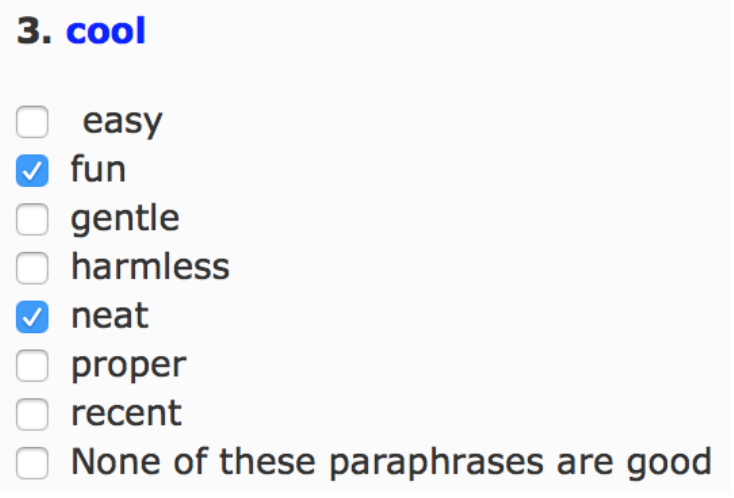
\includegraphics[width=\columnwidth]{hit.png}}%
% 	}%
% 	\caption{MTurk HIT for assessing goodness of paraphrases (without adverbs)}
% \end{figure}

% To select cut-off scores, we first developed and collected data from an MTurk HIT that asked workers to vote ``yes" or ``no" on the goodness of each presented paraphrase relationship (Figure 7). One version of the HIT did not include adverbs (i.e., workers assessed vertex pairs), and another version of the HIT included adverbs (i.e., workers assessed edges). Each vertex pair has at least one and potentially many associated edges. We asked workers to assess  10\% of the vertex pairs (randomly selected) and all of the corresponding edges. Each vertex pair or edge was judged by three workers, and their responses were used to take a majority vote. The majority votes were used as labels (either ``good" or ``bad") for each vertex pair or edge. Interestingly, we found that the majority votes of the edges tended to agree with the majority votes of their corresponding vertex pairs. That is, 1,150 of the majority votes for edges and vertex pairs were in agreement, while 461 were not in agreement. The Fleiss' kappa for the HIT without adverbs was 0.39, and the Fleiss' kappa for the HIT with adverbs was 0.29.

% \begin{figure}[t]
% 	{%
% 		\setlength{\fboxsep}{0pt}%
% 		\setlength{\fboxrule}{0.5pt}%
% 		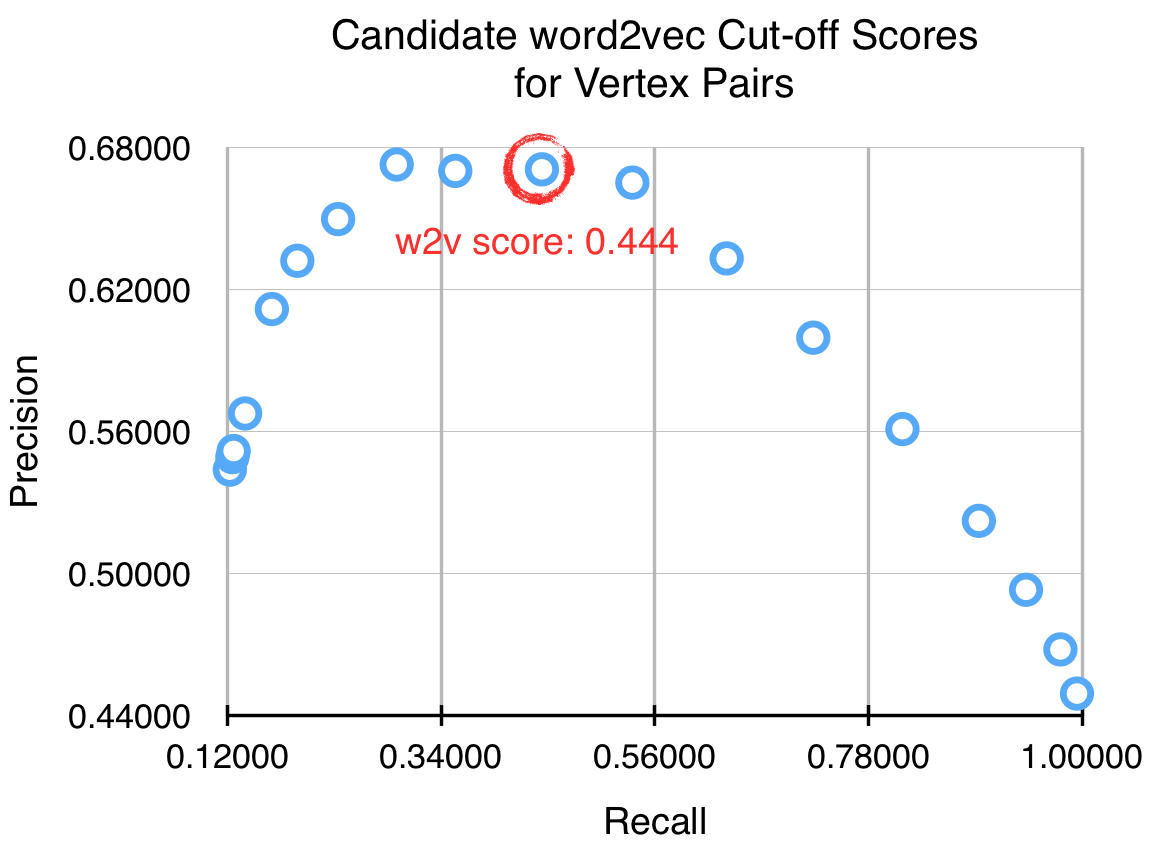
\includegraphics[width=\columnwidth]{w2v_cutoff_vertex_pairs.png}%
% 	}%
% 	\caption{Precision and recall for vertex pair \texttt{word2vec} cut-off scores}
% \end{figure}

% \begin{figure}[t]
% 	{%
% 		\setlength{\fboxsep}{0pt}%
% 		\setlength{\fboxrule}{0.5pt}%
% 		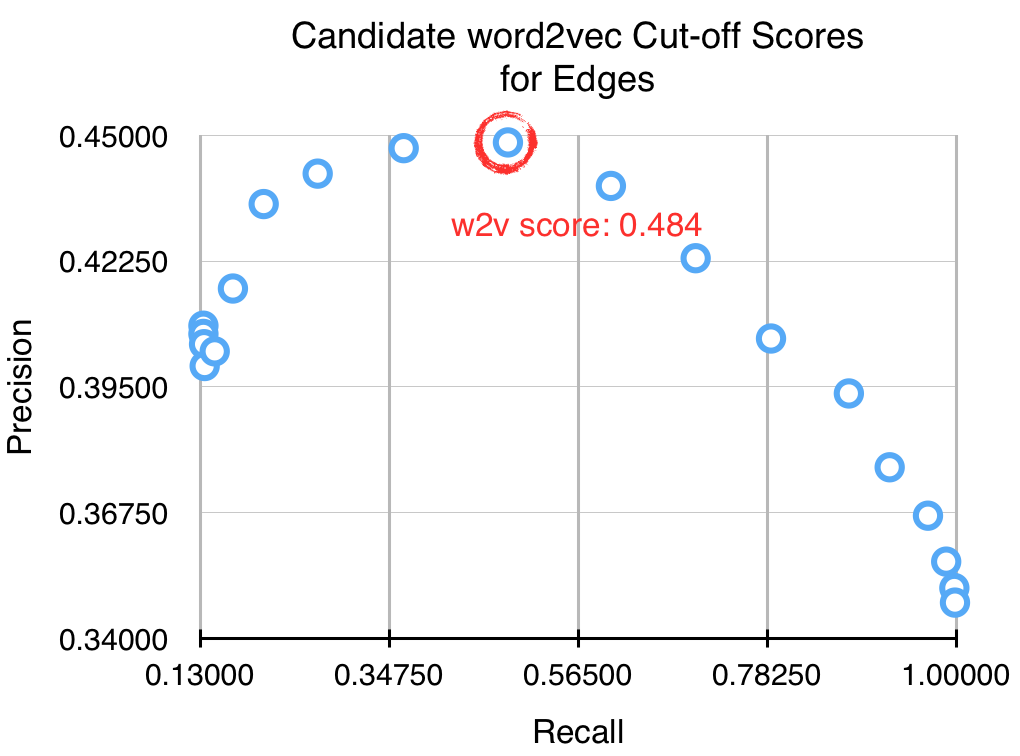
\includegraphics[width=\columnwidth]{w2v_cutoff_edges.png}%
% 	}%
% 	\caption{Precision and recall for edge \texttt{word2vec} cut-off scores}
% \end{figure}

% \begin{figure}[t]
% 	{%
% 		\setlength{\fboxsep}{0pt}%
% 		\setlength{\fboxrule}{0.5pt}%
% 		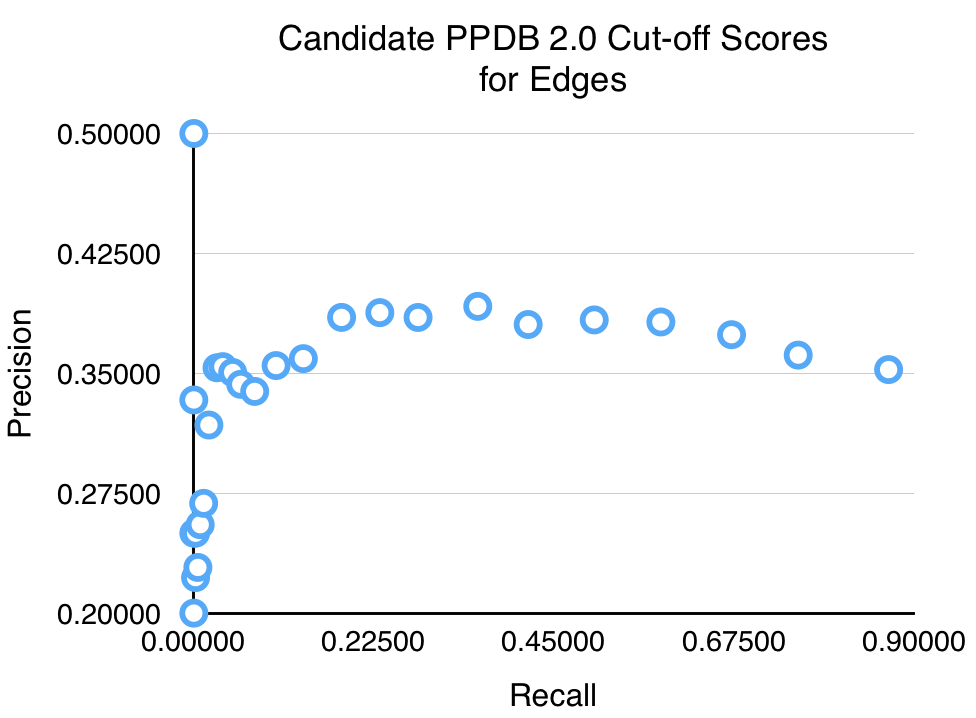
\includegraphics[width=\columnwidth]{ppdb2p0_cutoff_edges.png}%
% 	}%
% 	\caption{Precision and recall for edge PPDB 2.0 cut-off scores}
% \end{figure}

% We actually selected cut-off scores by formulating edge and vertex pair pruning as information retrieval tasks, and then selecting the score that performed the best on each task as the cut-off. The ``best" score is the one that has the highest precision with as little loss in recall as possible. Consider edge pruning. Each edge is ``good" (keep it in JJGraph) or ``bad" (remove it from JJGraph). The actual label (``good" or ``bad") for each edge is the Turkers' majority vote. If an edge's score is below the cut-off, its predicted label is ``bad." If an edge's score is above the cut-off, its predicted label is ``good." Thus, we can calculate the precision and recall of each candidate cut-off score. Pruning vertex pairs can be formulated as an analogous information retrieval task.

% Using this method, we calculated the precision and recall for vertex pair pruning and edge pruning at 20 \texttt{word2vec} scores in the range [0.05, 1.00]. We also calculated the precision and recall for edge pruning at 33 PPDB 2.0 scores in the range [3.60, 5.20] (the minimum and maximum PPDB 2.0 scores, respectively, among the sampled edges). See Figures 8-10 for these results. For vertex pairs, a \texttt{word2vec} score of $S_1 = 0.444$ was found to be the best cut-off. For edges, a \texttt{word2vec} score of $S_2 = 0.484$ was found to be the best cut-off. We found that PPDB 2.0 scores were not as reliable as \texttt{word2vec} scores (see Figure 10), so we opted to discard it as a goodness metric.

% 	Using the cut-off scores, we constructed 2 new graphs: (1) JJGraph$_\text{or}$, which consists of the edges that meet one (but not necessarily both) cut-off scores, and (2) JJGraph$_\text{and}$, which consists of the edges that meet both cut-off scores.
	
% 	More precisely, if $u$ and $v$ are adjectives that are related by an intensifying adverb $i$ in JJGraph, then let $\wsim(u, v)$ denote the word2vec similarity of the adjective $u$ and the adjective $v$, and let $\wsim_i(u, v)$ denote the similarity of adjectival phrase $i \text{ } u$ and the adjective $v$. JJGraph$_\text{or}$ contains the edge $(u, v)_i$ if $sim(u, v) > 0.444$ \textit{or} $sim_i(u, v) > 0.484$. JJGraph$_\text{and}$ contains the edge $(u, v)_i$ if $\wsim(u, v) > 0.444$ \textit{and} $\wsim_i(u, v) > 0.484$.
	
% 	The total number of edges in JJGraph, JJGraph$_\text{or}$, and JJGraph$_\text{and}$ are as follows: 
	
% 	\begin{center}
% 	\begin{tabular}{ |c|c|c| } 
%  	\hline
%  	Graph name & \# of edges \\ 
% 	\hline
%  	JJGraph & 36,756 \\ 
%  	JJGraph$_\text{or}$ & 19,370 \\ 
% 	JJGraph$_\text{and}$ & 13,185 \\
%  	\hline
% 	\end{tabular}
% 	\end{center}
	
% 	We will use JJGraph, JJGraph$_\text{or}$, and JJGraph$_\text{and}$ in the course of our research.


\section{Clustering adjectives in the graph}

Our first goal is to retrieve clusters of adjectives from \textit{JJGraph} that describe the same attribute as an (\textit{adjective, noun}) pair given as input. For example, given the pair (\textit{hot, coffee}), correct output would be a set of adjectives describing liquid temperature, such as \textit{warm}, \textit{lukewarm}, and \textit{scalding}.

The reason that we require an (\textit{adjective}, \textit{noun}) pair as input, rather than simply an \textit{adjective}, is that many adjectives are ambiguous. \textit{Hot}, for example, can describe temperature, but can also be used to describe appearance or popularity. Specifying a noun as part of the input serves to disambiguate the adjective.

Our adjective extraction process consists of three steps: first, filtering adjectives connected to the input adjective in \textit{JJGraph}; second, clustering the connected adjectives to disambiguate sense; and third, selecting the ``best-fit" cluster given the input noun. Here we describe each step in more detail.

\subsubsection{Filtering connected adjectives}

Given an input (\textit{adjective}, \textit{noun}) pair, call it $(j,n)$, our first step extracts adjectives from \textit{JJGraph} that (a) are directly connected to the adjective $j$ by a single (undirected) edge in \textit{JJGraph}, and (b) have been used to modify the noun $n$ in a corpus. The first criterion assumes that directly-connected adjectives can be used to describe the same attribute. The second criterion serves to filter out adjectives that do not describe the same attribute.

The corpus we use for this step and the next is a set of business reviews from the Yelp Dataset Challenge \cite{yelpdataset}. This set of 2.6M reviews covering 86K businesses is useful because it contains many instances of adjectives of varying intensity that modify a single attribute (such as food taste, or service speed).
%can we quantify this somehow?
When filtering adjectives connected to $j$ in \textit{JJGraph}, we retain all directly-connected $j^\prime$ that have modified $n$ at least ten times in the Yelp corpus, and are also highly associated with $n$. We quantify the level of association between an adjective-noun pair $(j,n)$ using (normalized) pointwise mutual information $nmi_{j,n}$, with a discounting factor $dsc_{j,n}$ to down-weight highly infrequent pairs \cite{pantel2002discovering}:

\[nmi_{j,n} = -\log_2(mi_{j,n} \times dsc_{j,n}) / nrm_{j,n}\]

\[mi_{j,n} = \frac{\frac{f(j,n)}{N}}{\frac{\sum_u f(u,n)}{N} \times \frac{\sum_v f(j,v)}{N}}\]

\[dsc_{j,n} = \frac{f(j,n)}{f(j,n)+1} \times \frac{min(\sum_u f(u,n), \sum_v f(j,v))}{min(\sum_u f(u,n), \sum_v f(j,v)) + 1}\]

\[nrm_{j,n} = -\log_2 \frac{f(j,n)}{N}\]

\noindent where $N=\sum_u \sum_v f(u,v)$ is the total frequency count of all adjective-noun pairs in the Yelp corpus.

When filtering adjectives, we require each $j^\prime$ to have $PMI(^\prime, n) > t$, where $t$ is a threshold parameter. In our experiments we vary $t \in \{0.0, 0.01, 0.1\}$.

\subsubsection{Clustering filtered adjectives}

Even after filtering adjectives to include only those known to modify the input noun, it is still possible to retrieve a set of adjectives describing multiple attributes. This is particularly true when the input adjective is polysemous. For example, the set of filtered adjectives returned for the query (\textit{hot,coffee}) includes \textit{fantastic, fabulous, spectacular}, and \textit{cold, lukewarm}, although only the last two are applicable in most contexts.

To counteract this result, we cluster the set of filtered adjectives by the sense of the target they convey. Using \textit{JJGraph} this is a simple process; we simply take the subgraph formed by removing all nodes from  \textit{JJGraph} except the set of filtered adjectives, and partition the resulting subgraph into connected components. This serves to divide the filtered adjectives into coarse sense clusters.

\subsubsection{Selecting the best cluster}

Given a set of one or more clusters of adjectives, the last step is to choose which cluster is most applicable to the original adjective-noun input pair. The most applicable cluster should contain adjectives $j^\prime$ that are (a) highly similar to the input adjective, $j$, and (b) highly associated with the input noun, $n$. Therefore we assign a score $s_c$ to each cluster, where

\[s_C = avg_{j^\prime \in C} nmi_{j^\prime,n} \times avg_{j^\prime \in C} PPDBScore_{j,j^\prime}\]

\noindent The mutual information, $nmi_{j^\prime, n}$ is calculated as before. The component $PPDBScore_{j,j^\prime}$ gives the PPDB 2.0 Score between adjectives.\footnote{PPDB2.0 Score is a supervised metric designed to correlated with human judgements of paraphrase quality \cite{pavlick-EtAl:2015:ACL-IJCNLP3}} 

The final cluster $\hat{C}$ returned by our algorithm is that which produces the maximum $s_C$.

% \subsection{Evaluation}

% We evaluate the adjectives returned by our method for an input (\textit{adjective},\textit{noun}) pair against two sets of ground truth clusters. The first is a manually-compiled dataset published by \newcite{demelo:13}, consisting of X \textit{target} adjectives and associated same-attribute adjectives for each target. In the original dataset the same-attribute adjectives are sorted by intensity, but we ignore their ordering for this cluster evaluation.

% Second, we separately generate our own set of ground-truth clusters with the help of crowd workers from Amazon Mechanical Turk (MTurk). Here we detail the dataset construction pipeline.

% \subsubsection{Ground Truth Cluster Creation}

% To quantitatively assess the goodness of generated adjective clusters, we compare them to a set of gold standard clusterings. A \textbf{clustering} is a set of one or more clusters associated with a target adjective. Each cluster within a clustering represents a semantic sense of the adjective, and thus the adjectives within a cluster can be ordered along a single scale of increasing intensity. We created the gold standard clusters in the course of this research. 

% Each clustering was constructed around a single adjective. For example, a gold standard clustering containing \textit{disgusting}, \textit{nasty}, and \textit{repulsive} might have been constructed around \textit{foul}. Clusters within clusterings do not need to be disjoint, as some adjectives have multiple senses (e.g., \textit{hot} may mean either \textit{warm} or \textit{attractive}). 

% We selected words with high centrality around which to create gold standard clusterings. We selected words with high centrality because such words are the most difficult to construct a good cluster for, given that such words have many possible senses. Thus, if our methods can construct a good cluster for an adjective with high centrality, then we should be able to construct a good cluster for any adjective in the graph. 

% We consider an adjective to have ``high centrality" if it is among the 200 most central words according to two of three centrality measurements -- betweenness centrality, closeness centrality, and degree centrality. With this criterion, we selected 145 adjectives (``target adjectives") around which adjective clusterings were generated. We  generated the clusters using two successive MTurk HITs. Candidate adjectives for each cluster were taken from the graph. For each of the 145 target adjectives, we generated a list of candidate cluster members by collecting the first 20 words encountered in a breadth-first search starting at the adjective in \textit{JJGraph}. 

% To construct a gold standard cluster for a target adjective, we first removed cluster candidates that did not belong on any scale with the target adjective. We experimented with several HIT designs, and ultimately settled on one that asked MTurk workers to determine whether pairs of adjectives described the same attribute (see Figure 4). Each pair consisted of a target adjective and a cluster candidate adjective. Three workers assessed each pair of adjectives. If a majority of workers declared that a pair of adjectives described the same attribute, then the candidate word was advanced to the next round.

% \begin{figure}[t]
% 	{%
% 		\setlength{\fboxsep}{0pt}%
% 		\setlength{\fboxrule}{0.5pt}%
% 		\fbox{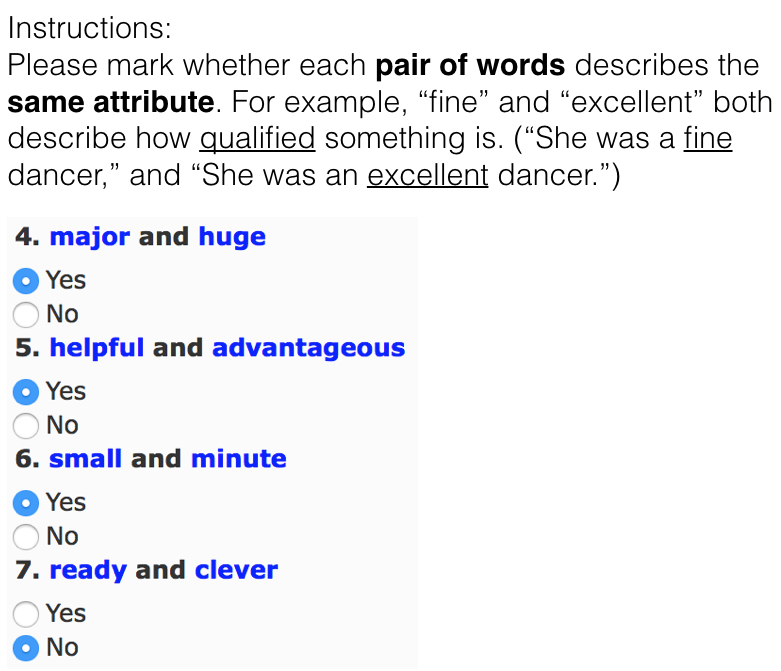
\includegraphics[width=\columnwidth]{hit_same_attribute.png}}%
% 	}%
% 	\caption{First MTurk HIT for constructing gold standard adjective clusters. Each question consists of a target adjective (left) and a cluster candidate adjective (right).}
% \end{figure} 

% In the second round, workers were asked to construct a clustering for a target adjective. Between 2 and 10 workers constructed a clustering for each target adjective. Once a predefined level of agreement was reached among workers for a target adjective's clustering, the clustering was deemed ``gold." 

% In total, we constructed gold standard clusterings for 145 adjectives. Each clustering has an average of 3.26 clusters.

% \begin{figure}[t]
% 	{%
% 		\setlength{\fboxsep}{0pt}%
% 		\setlength{\fboxrule}{0.5pt}%
% 		\fbox{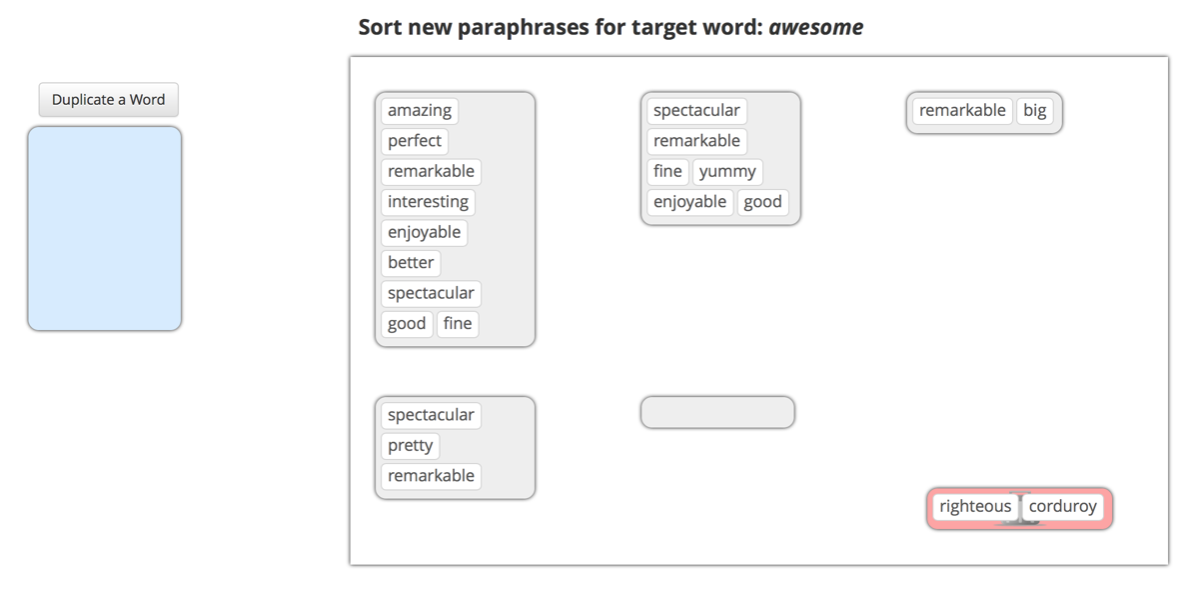
\includegraphics[width=\columnwidth]{hit_cluster.png}}%
% 	}%
% 	\caption{Second MTurk HIT for constructing gold standard adjective clusters.}
% \end{figure} 

% \subsubsection{Evaluating automatically constructed adjective clusters}

% To evaluate our system, we compare our automatically extracted adjective clusters to the aforementioned gold standard clusterings. Both gold standard datasets consist of tuples of (\textit{target}, \textit{cluster}) pairs, where each \textit{target} is an adjective and each \textit{cluster} consists of additional adjectives describing the same attribute. We evaluate our clusters against these ground-truth examples in order to determine (1) whether our algorithm retrieves adjectives of the correct sense given a (JJ, NN) pair with a polysemous adjective, and (2) to what extent the retrieved clusters align with the ground-truth ones.

% Our evaluation pipeline is as follows. For each ($JJ^\star$, $C$) tuple in the ground-truth dataset, where $JJ^\star$ is the target adjective and $C$ is the gold standard adjective cluster, we first select a prototypical noun, $NN^\star$ that pertains to the attribute described by the gold cluster. To do this, we find the noun in the Yelp dataset having the highest average frequency with $JJ^\star$ and all words in $C$. For example, if the ground truth tuple is (\textit{long}, \{\textit{time-consuming}, \textit{lengthy}, \textit{long-standing}\}), a prototypical noun might be \textit{meeting}. 

% Next, we retrieve adjectives using our method for the input $(JJ^\star, NN^\star)$, and evaluate the result using the following metrics:

% \begin{itemize}
% \item \textbf{Match}: a binary metric indicating whether the `best-fit' cluster chosen by our algorithm has highest overlap among all possible clusters with the ground truth $C$.
% \item \textbf{Precision}: measures the percent of words in the `best-fit' cluster chosen by our algorithm that appear in the ground truth cluster. 
% \item \textbf{Recall}: measures the percent of words in the ground truth cluster (also appearing in \textit{JJGraph}) that appear in the `best-fit' cluster.
% \end{itemize}

% We compare our method to two baselines. The first, \textit{Connected}, returns as the best-fit cluster the set of all adjectives connected to $JJ^\star$ in \textit{JJGraph} by a path of length one. The second, \textit{Connected-Filtered}, returns as the best-fit cluster the same set as \textit{Connected}, but also filtered to exclude adjectives that do not appear with $NN^\star$ in the Yelp dataset with minimum frequency 10 or minimum  mutual information $nmi_{JJ,NN^\star}$ above a threshold.

% \subsubsection{Results}

% The results of our adjective extraction method, as compared to both gold standard datasets, are given in Table \ref{tab:clustering-results}.

% \begin{table}[]
% \centering
% \begin{tabular}{@{}llll@{}}
% \toprule
% Method             & Match & Precision & Recall \\ \midrule
% \multicolumn{4}{c}{Dataset: Crowd Clusters}     \\ \midrule
% \textit{Connected }         &       &           &        \\
% \textit{Connected-Filtered} &       &           &        \\
% \textit{Clustered}             &       &           &        \\
% \multicolumn{4}{c}{Dataset: DeMelo et al.}      \\ \midrule
% \textit{Connected}          &       &           &        \\
% \textit{Connected-Filtered} &       &           &        \\
% \textit{Clustered}             &       &           &        \\
% \end{tabular}
% \caption{Results of adjective retrieval evaluation, with minimum \textit{nmi} threshold 0.1. Scores reported are weighted averages over all tuples in each ground-truth dataset, where the weight for each ground-truth sample is the size of the ground-truth cluster.}
% \label{tab:clustering-results}
% \end{table}

\subsection{Qualitative Evaluation}

We qualitatively examine the adjective clusters retrieved by our methods.

\begin{table}[]
\centering
\begin{tabular}{@{}lll@{}}
\toprule
Method & Query & Result \\ \midrule

\bottomrule
\end{tabular}
\caption{Clusters retrieved for various queries by our method.}
\label{tab:clustering-qual-results}
\end{table}


%##TODO: Include table of qualitative results



\section{Ordering adjectives by intensity}

% TODO: Write this

\section{Application: Predicting aspect-based sentiment polarity}

% TODO: Write this

%\section{Application: Predicting spam reviews}
% TODO: Write this if there's room and time

\section{Conclusion}

In this work, we have presented our progress towards developing a pipeline to cluster semantically similar adjectives and to rank adjectives within a cluster according to their relative intensity. Future work will include further experimentation with clustering algorithms and developing algorithms to rank related adjectives within a cluster on a scale

% \section*{Acknowledgments}

% The acknowledgments should go immediately before the references.  Do
% not number the acknowledgments section. Do not include this section
% when submitting your paper for review.

% include your own bib file like this:
%\bibliographystyle{acl}
%\bibliography{naaclhlt2018}
\bibliography{scalar-adj}
\bibliographystyle{acl_natbib}

% \appendix

% \section{Supplemental Material}
% \label{sec:supplemental}


\end{document}
